\documentclass{standalone}
\usepackage{tikz}
\usetikzlibrary{patterns, positioning}
\usepackage[sfdefault]{ClearSans} %% option 'sfdefault' activates Clear Sans as the default text font
\usepackage[T1]{fontenc}

\begin{document}
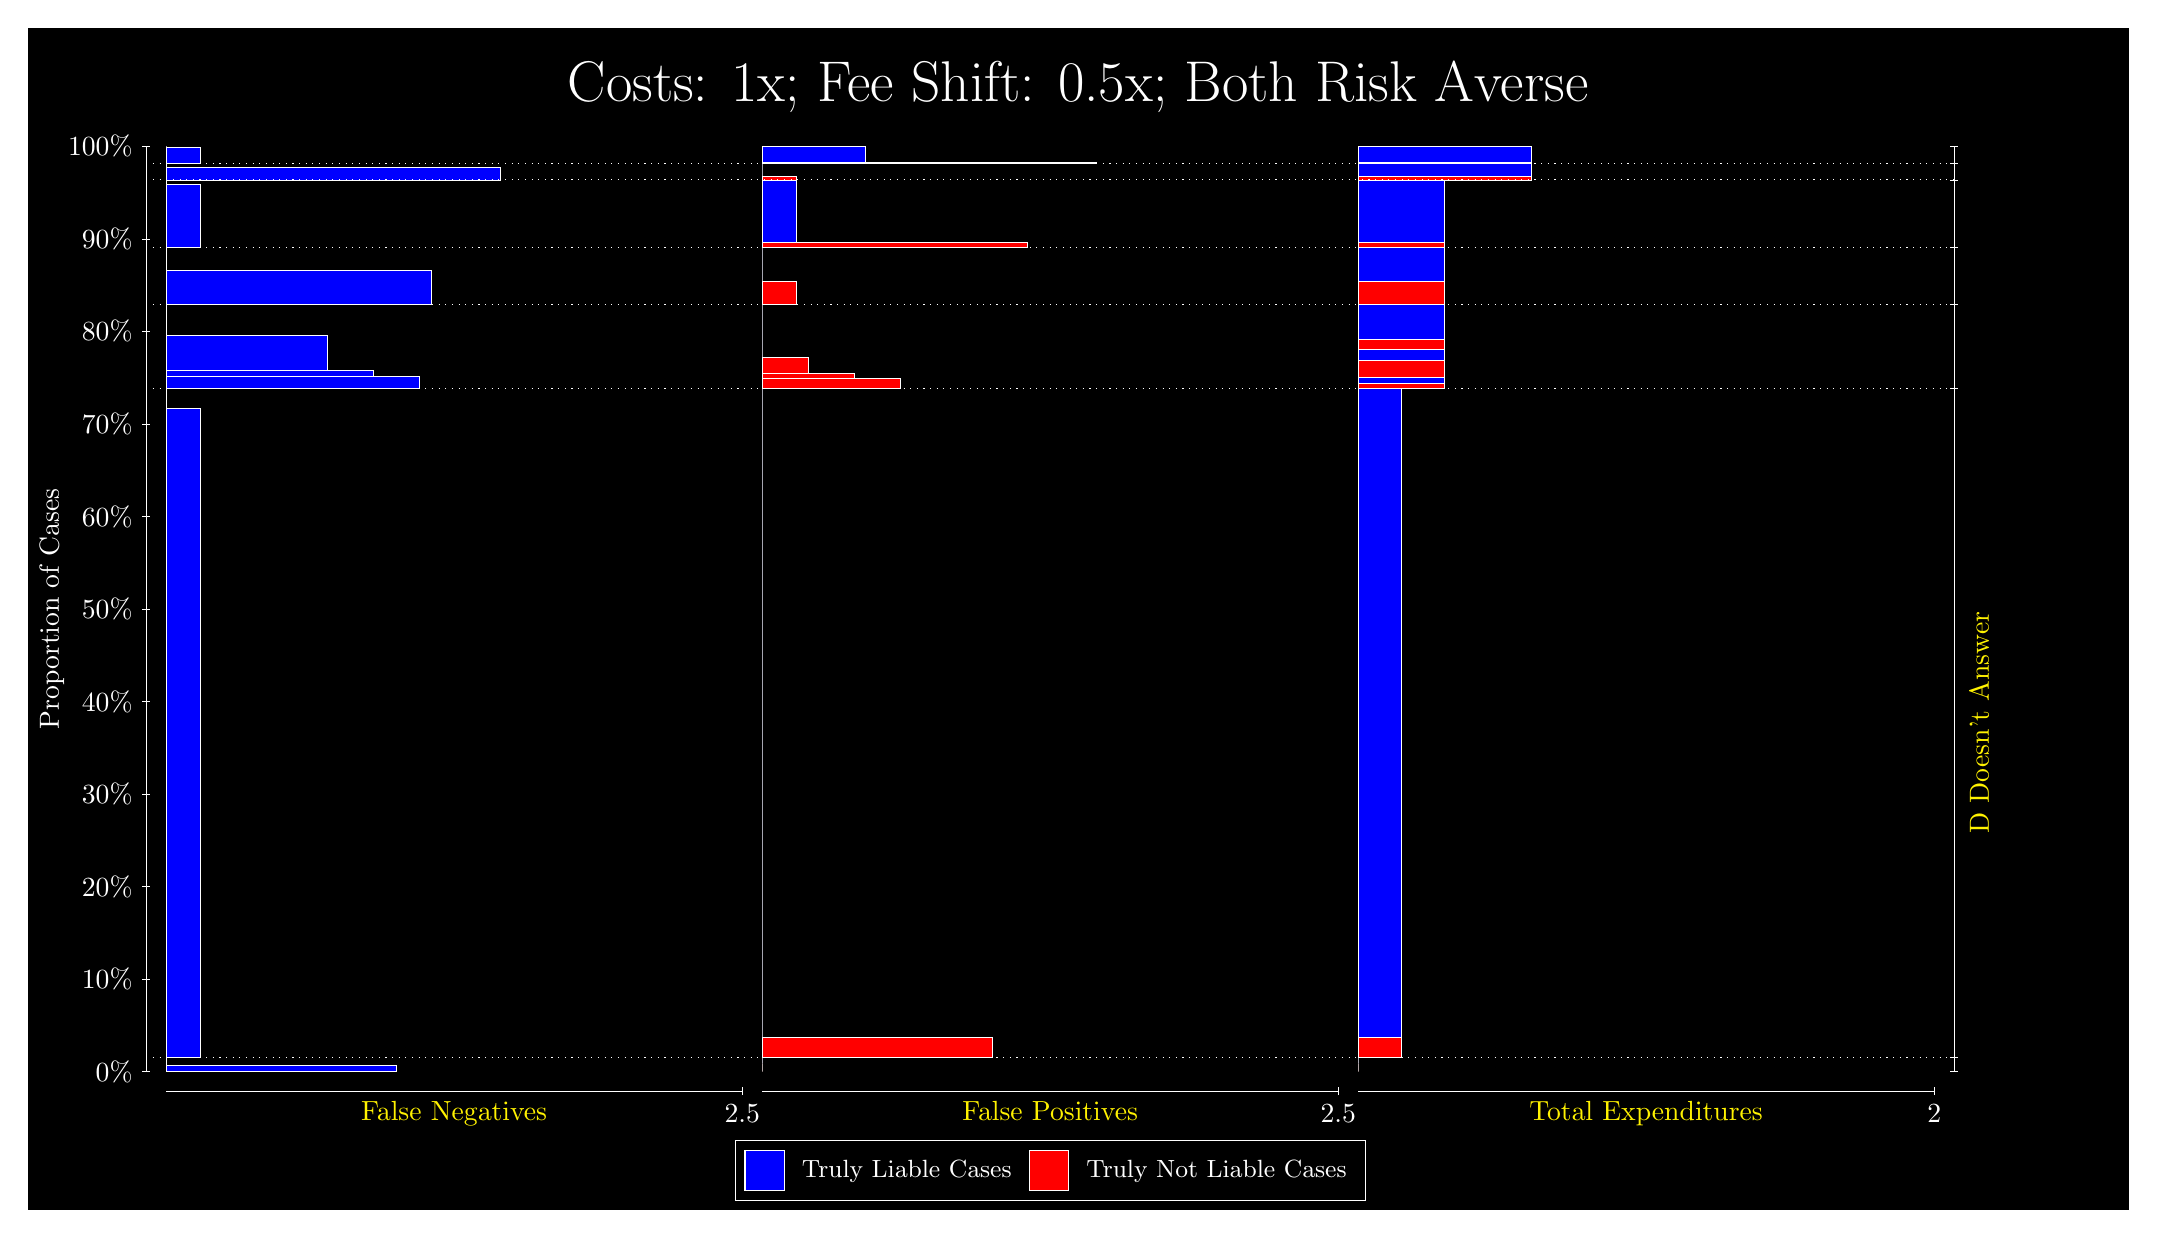
\begin{tikzpicture}
\draw[fill=black] (0,0) rectangle (26.667,15);
\draw[text=white] (0,13.5) rectangle (26.667,15) node[midway] {\huge Costs: 1x; Fee Shift: 0.5x; Both Risk Averse};
\draw[white, very thin] (1.5,1.75) -- (1.5,13.5);
\node[rotate=90, text=white, anchor=center] at (0.3, 7.625) {Proportion of Cases};
\draw[white, very thin] (1.45,1.75) -- (1.55,1.75);
\node[text=white, anchor=east] at (1.45, 1.75) {0\%};
\draw[white, very thin] (1.45,2.925) -- (1.55,2.925);
\node[text=white, anchor=east] at (1.45, 2.925) {10\%};
\draw[white, very thin] (1.45,4.1) -- (1.55,4.1);
\node[text=white, anchor=east] at (1.45, 4.1) {20\%};
\draw[white, very thin] (1.45,5.275) -- (1.55,5.275);
\node[text=white, anchor=east] at (1.45, 5.275) {30\%};
\draw[white, very thin] (1.45,6.45) -- (1.55,6.45);
\node[text=white, anchor=east] at (1.45, 6.45) {40\%};
\draw[white, very thin] (1.45,7.625) -- (1.55,7.625);
\node[text=white, anchor=east] at (1.45, 7.625) {50\%};
\draw[white, very thin] (1.45,8.8) -- (1.55,8.8);
\node[text=white, anchor=east] at (1.45, 8.8) {60\%};
\draw[white, very thin] (1.45,9.975) -- (1.55,9.975);
\node[text=white, anchor=east] at (1.45, 9.975) {70\%};
\draw[white, very thin] (1.45,11.15) -- (1.55,11.15);
\node[text=white, anchor=east] at (1.45, 11.15) {80\%};
\draw[white, very thin] (1.45,12.325) -- (1.55,12.325);
\node[text=white, anchor=east] at (1.45, 12.325) {90\%};
\draw[white, very thin] (1.45,13.5) -- (1.55,13.5);
\node[text=white, anchor=east] at (1.45, 13.5) {100\%};

\draw[white, very thin] (24.457,1.75) -- (24.457,13.5);
\draw[white, very thin] (24.407,1.75) -- (24.507,1.75);
\node[anchor=west] at (24.407, 1.75) {};
\draw[white, very thin] (24.407,1.9332) -- (24.507,1.9332);
\node[anchor=west] at (24.407, 1.9332) {};
\draw[white, very thin] (24.407,10.427) -- (24.507,10.427);
\node[anchor=west] at (24.407, 10.427) {};
\draw[white, very thin] (24.407,11.491) -- (24.507,11.491);
\node[anchor=west] at (24.407, 11.491) {};
\draw[white, very thin] (24.407,12.219) -- (24.507,12.219);
\node[anchor=west] at (24.407, 12.219) {};
\draw[white, very thin] (24.407,13.074) -- (24.507,13.074);
\node[anchor=west] at (24.407, 13.074) {};
\draw[white, very thin] (24.407,13.282) -- (24.507,13.282);
\node[anchor=west] at (24.407, 13.282) {};
\draw[white, very thin] (24.407,13.5) -- (24.507,13.5);
\node[anchor=west] at (24.407, 13.5) {};

\draw[white, very thin, fill=blue] (1.75,1.75) rectangle (4.6775,1.831);
\draw[white, very thin, fill=red] (1.75,1.831) rectangle (1.75,1.9332);
\draw[white, very thin, fill=blue] (1.75,1.9332) rectangle (2.1891,10.177);
\draw[white, very thin, fill=red] (1.75,10.177) rectangle (1.75,10.427);
\draw[white, very thin, fill=blue] (1.75,10.427) rectangle (4.9703,10.574);
\draw[white, very thin, fill=blue] (1.75,10.574) rectangle (4.3848,10.658);
\draw[white, very thin, fill=blue] (1.75,10.658) rectangle (3.7993,11.095);
\draw[white, very thin, fill=red] (1.75,11.095) rectangle (1.75,11.491);
\draw[white, very thin, fill=blue] (1.75,11.491) rectangle (5.1167,11.921);
\draw[white, very thin, fill=red] (1.75,11.921) rectangle (1.75,12.219);
\draw[white, very thin, fill=blue] (1.75,12.219) rectangle (2.1891,13.014);
\draw[white, very thin, fill=red] (1.75,13.014) rectangle (1.75,13.074);
\draw[white, very thin, fill=blue] (1.75,13.074) rectangle (5.9949,13.232);
\draw[white, very thin, fill=red] (1.75,13.232) rectangle (1.75,13.282);
\draw[white, very thin, fill=blue] (1.75,13.282) rectangle (2.1891,13.482);
\draw[white, very thin, fill=red] (1.75,13.482) rectangle (1.75,13.5);
\draw[white, very thin, fill=red] (9.3189,1.75) rectangle (9.3189,1.8522);
\draw[white, very thin, fill=blue] (9.3189,1.8522) rectangle (9.3189,1.9332);
\draw[white, very thin, fill=red] (9.3189,1.9332) rectangle (12.246,2.1835);
\draw[white, very thin, fill=blue] (9.3189,2.1835) rectangle (9.3189,10.427);
\draw[white, very thin, fill=red] (9.3189,10.427) rectangle (11.075,10.553);
\draw[white, very thin, fill=red] (9.3189,10.553) rectangle (10.49,10.612);
\draw[white, very thin, fill=red] (9.3189,10.612) rectangle (9.9044,10.824);
\draw[white, very thin, fill=blue] (9.3189,10.824) rectangle (9.3189,11.491);
\draw[white, very thin, fill=red] (9.3189,11.491) rectangle (9.758,11.789);
\draw[white, very thin, fill=blue] (9.3189,11.789) rectangle (9.3189,12.219);
\draw[white, very thin, fill=red] (9.3189,12.219) rectangle (12.686,12.279);
\draw[white, very thin, fill=blue] (9.3189,12.279) rectangle (9.758,13.074);
\draw[white, very thin, fill=red] (9.3189,13.074) rectangle (9.758,13.124);
\draw[white, very thin, fill=blue] (9.3189,13.124) rectangle (9.3189,13.282);
\draw[white, very thin, fill=red] (9.3189,13.282) rectangle (13.564,13.3);
\draw[white, very thin, fill=blue] (9.3189,13.3) rectangle (10.636,13.5);
\draw[white, very thin, fill=red] (16.888,1.75) rectangle (16.888,1.8522);
\draw[white, very thin, fill=blue] (16.888,1.8522) rectangle (16.888,1.9332);
\draw[white, very thin, fill=red] (16.888,1.9332) rectangle (17.437,2.1835);
\draw[white, very thin, fill=blue] (16.888,2.1835) rectangle (17.437,10.427);
\draw[white, very thin, fill=red] (16.888,10.427) rectangle (17.986,10.486);
\draw[white, very thin, fill=blue] (16.888,10.486) rectangle (17.986,10.569);
\draw[white, very thin, fill=red] (16.888,10.569) rectangle (17.986,10.781);
\draw[white, very thin, fill=blue] (16.888,10.781) rectangle (17.986,10.928);
\draw[white, very thin, fill=red] (16.888,10.928) rectangle (17.986,11.054);
\draw[white, very thin, fill=blue] (16.888,11.054) rectangle (17.986,11.491);
\draw[white, very thin, fill=red] (16.888,11.491) rectangle (17.986,11.789);
\draw[white, very thin, fill=blue] (16.888,11.789) rectangle (17.986,12.219);
\draw[white, very thin, fill=red] (16.888,12.219) rectangle (17.986,12.279);
\draw[white, very thin, fill=blue] (16.888,12.279) rectangle (17.986,13.074);
\draw[white, very thin, fill=red] (16.888,13.074) rectangle (19.083,13.124);
\draw[white, very thin, fill=blue] (16.888,13.124) rectangle (19.083,13.282);
\draw[white, very thin, fill=red] (16.888,13.282) rectangle (19.083,13.3);
\draw[white, very thin, fill=blue] (16.888,13.3) rectangle (19.083,13.5);
\draw[white, dotted] (1.5,1.9332) -- (24.457,1.9332);
\draw[white, dotted] (1.5,10.427) -- (24.457,10.427);
\draw[white, dotted] (1.5,11.491) -- (24.457,11.491);
\draw[white, dotted] (1.5,12.219) -- (24.457,12.219);
\draw[white, dotted] (1.5,13.074) -- (24.457,13.074);
\draw[white, dotted] (1.5,13.282) -- (24.457,13.282);
\draw[white, very thin] (1.75,1.5) -- (9.0689,1.5);
\node[text=yellow, anchor=north] at (5.4094, 1.5) {False Negatives};
\draw[white, very thin] (9.0689,1.45) -- (9.0689,1.55);
\node[text=white, anchor=north] at (9.0689, 1.45) {2.5};

\draw[white, very thin] (9.3189,1.5) -- (16.638,1.5);
\node[text=yellow, anchor=north] at (12.978, 1.5) {False Positives};
\draw[white, very thin] (16.638,1.45) -- (16.638,1.55);
\node[text=white, anchor=north] at (16.638, 1.45) {2.5};

\draw[white, very thin] (16.888,1.5) -- (24.207,1.5);
\node[text=yellow, anchor=north] at (20.547, 1.5) {Total Expenditures};
\draw[white, very thin] (24.207,1.45) -- (24.207,1.55);
\node[text=white, anchor=north] at (24.207, 1.45) {2};


\node[text=yellow, centered, rotate=90] at (24.777, 6.1802) {D Doesn't Answer};






\draw (12.978300999999998,1.5) node[draw=none] (baseCoordinate) {};
\begin{scope}[align=center]
        \matrix[scale=0.5, draw=white, below=0.5cm of baseCoordinate, nodes={draw}, column sep=0.1cm]{
            \node[rectangle, draw, minimum width=0.5cm, minimum height=0.5cm, fill=blue] {}; &
            \node[draw=none, font=\small, text=white] (B) {Truly Liable Cases}; &
            \node[rectangle, draw, minimum width=0.5cm, minimum height=0.5cm, fill=red] {}; &
            \node[draw=none, font=\small, text=white] (B) {Truly Not Liable Cases}; \\
            };
\end{scope}

\end{tikzpicture}
\end{document}